% Five-Stage Pipeline TikZ Diagram
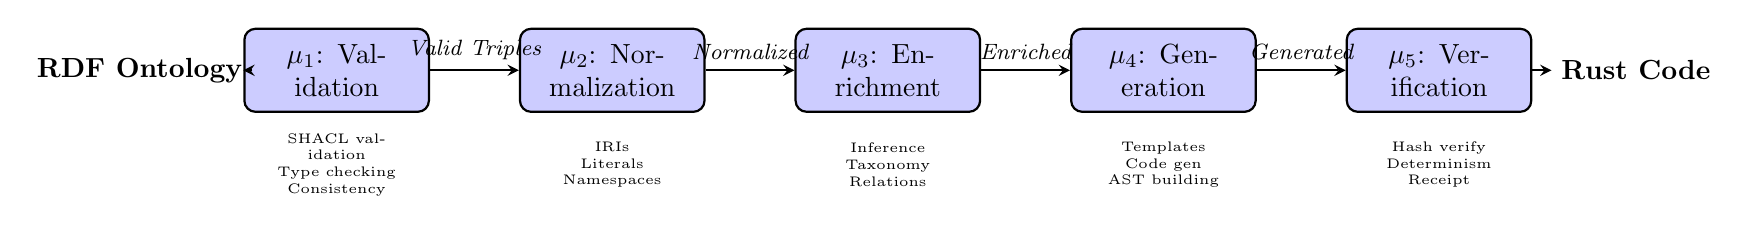
\begin{tikzpicture}[
    node distance=1.5cm,
    auto,
    block/.style={
        rectangle,
        draw,
        fill=blue!20,
        text width=6em,
        text centered,
        rounded corners,
        minimum height=3em,
        thick
    },
    arrow/.style={
        ->,
        thick,
        >=stealth
    },
    label/.style={
        font=\footnotesize\itshape
    }
]

% Nodes
\node [block] (mu1) {$\mu_1$: Validation};
\node [block, right of=mu1, node distance=3.5cm] (mu2) {$\mu_2$: Normalization};
\node [block, right of=mu2, node distance=3.5cm] (mu3) {$\mu_3$: Enrichment};
\node [block, right of=mu3, node distance=3.5cm] (mu4) {$\mu_4$: Generation};
\node [block, right of=mu4, node distance=3.5cm] (mu5) {$\mu_5$: Verification};

% Input/Output
\node [left of=mu1, node distance=2.5cm] (input) {\textbf{RDF Ontology}};
\node [right of=mu5, node distance=2.5cm] (output) {\textbf{Rust Code}};

% Arrows
\draw [arrow] (input) -- (mu1);
\draw [arrow] (mu1) -- node[above, label] {Valid Triples} (mu2);
\draw [arrow] (mu2) -- node[above, label] {Normalized} (mu3);
\draw [arrow] (mu3) -- node[above, label] {Enriched} (mu4);
\draw [arrow] (mu4) -- node[above, label] {Generated} (mu5);
\draw [arrow] (mu5) -- (output);

% Stage descriptions
\node [below of=mu1, node distance=1.2cm, text width=5em, align=center, font=\tiny] {
    SHACL validation\\
    Type checking\\
    Consistency
};

\node [below of=mu2, node distance=1.2cm, text width=5em, align=center, font=\tiny] {
    IRIs\\
    Literals\\
    Namespaces
};

\node [below of=mu3, node distance=1.2cm, text width=5em, align=center, font=\tiny] {
    Inference\\
    Taxonomy\\
    Relations
};

\node [below of=mu4, node distance=1.2cm, text width=5em, align=center, font=\tiny] {
    Templates\\
    Code gen\\
    AST building
};

\node [below of=mu5, node distance=1.2cm, text width=5em, align=center, font=\tiny] {
    Hash verify\\
    Determinism\\
    Receipt
};

\end{tikzpicture}
